\section{Future work: integration of DVMS with OpenStack}
\label{sec:future_work}

\subsection{DVMS: a dynamic scheduler for virtual machines}

% \begin{itemize}

% 	\item Dynamic scheduler for virtual machines.

% 	\item Leverage a locality aware p2p overlay.

% 	\item Successfuly tested in simulator (simgrid) and computing grid (grid'5000).

% \end{itemize}

DVMS \cite{quesnel:ispa2013} (Distributed Virtual Machine Scheduler) is a
ressource scheduler that cooperatively and dynamically ensures virtual machines
hosted in large scale infrastructure meet their computing ressources needs. DVMS
treats ressources overloading as a bin packing problem: when a DVMS agent cannot
guarantee its virtual machines needs, it tries to find suitable collaborators 
that will help to make a viable virtual machines placement.

To resolve a ressource overload, a DVMS agent create and join a partition and
forward it to a remote DVMS agent that is not already belonging to a partition.
This remote free agent will first join the partition and then begin to compute 
for a viable mapping. In the case where the computation is unsuccesful, the new 
version of the partition is forwarded to another free DVMS agent until a viable
mapping is found. When a viable mapping has been found, the last member of the
partition applies the mapping by performing live virtual machines migrations.

Formal proof \cite{quesnel:ispa2013} has been made that if a solution exits, 
DVMS will converge to this solution. Furthermore, as a DVMS agent cannot be
shared between different partitions, partitions can work in parallel without
lock mechanisms, thus improving DVMS reactivity. Finally experiments conducted 
on grid5000' testbed have shown that independantly from the infrastructure 
size, partitions only involve few nodes thus limiting the network overhead 
caused by communications.


\subsection{Integration of DVMS in OpenStack}

\label{sub:sec:integration_dvms}

% \begin{itemize}

% \item We propose to replace "nova-scheduler" (static scheduler) by DVMS.

% \item Use of an "Adapter" object that will wrap DVMS and integrate well with OpenStack, as described in figure \ref{fig:integration}
% 	\begin{itemize}
% 		\item It will consume messages that are destinated to "nova-scheduler"

% 		\item Each message will be converted to a "Dvms" message.

% 		\item Each message produced by Dvms will be converted to an OpenStack message and added to the Queue.

% 	\end{itemize}
% \end{itemize}


Considering the fact that nova-scheduler currently performs static scheduling, 
as introduced in section \ref{sub:sec:revisiting_openstack}, we decided to 
replace it by DVMS. Before going more into technical details of the integration,
OpenStack's service architecture is flexible: service follow the "shared nothing
memory" principle and communicate through an AMQP bus. This means that each 
service follows a "protocol" : when it consumes all received message, in return
it execute an action and produces a specific messsage. 

\begin{figure}[h]
	\centering
	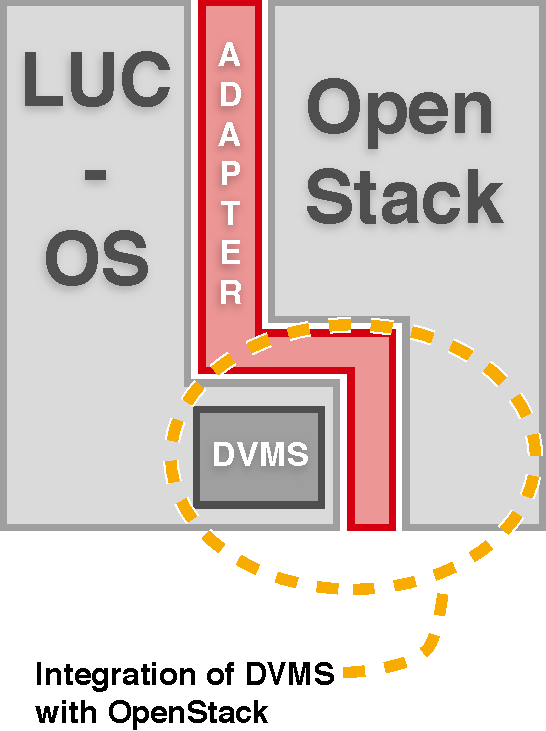
\includegraphics[width=0.50\linewidth]{Figures/dvms_openstack.pdf}
	\caption{Integration of DVMS in OpenStack.}%
	\label{fig:integration}%
	%\vspace*{-.8cm}
\end{figure}

With this in mind, we depicted in figure \ref{fig:integration} the way we want 
to integrate DVMS with OpenStack: we use an adapter object that consumes 
messages that are destinated to nova-scheduler, forward it to DVMS and translate
messages produced by DMVS in message from the nova-scheduler protocol. We think
that this method will minimize modification on Nova service.
